\documentclass[tikz,border=2pt]{standalone}
\usepackage{amsmath}
\usepackage{pgfplots}
\pgfplotsset{compat=1.18}

\begin{document}
% b^x for b=2 (growth) and b=1/2 (decay): both pass through (0,1), stay positive and
% have the x-axis as a horizontal asymptote on one side.
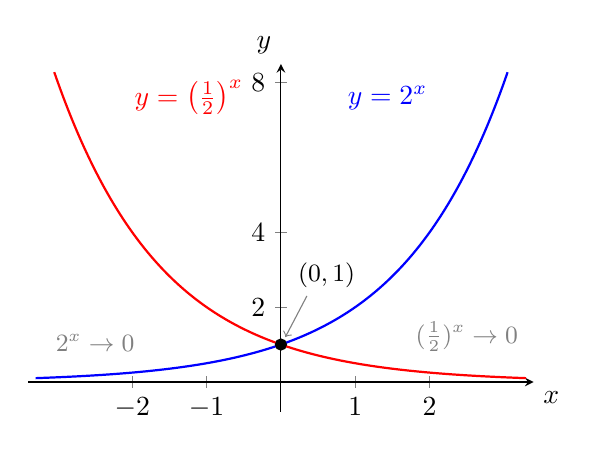
\begin{tikzpicture}
	\begin{axis}[
		axis lines=middle,
		xmin=-3.4, xmax=3.4,
		ymin=-0.8, ymax=8.5,
		xtick={-2,-1,1,2}, ytick={2,4,8},
		xlabel={$x$}, ylabel={$y$},
		xlabel style={below right}, ylabel style={above left},
		samples=120, smooth, clip=false,
		width=8cm, height=6cm
		]
		\addplot[thick, blue, domain=-3.3:3.05] {2^x};
		\addplot[thick, red, domain=-3.05:3.3] {0.5^x};
		\addplot[only marks, mark=*, black] coordinates {(0,1)};
		\node[anchor=south west, font=\small] at (axis cs:0.1,2.25) {$(0,1)$};
		\draw[gray, ->] (axis cs:0.35,2.3) -- (axis cs:0.06,1.2);
		\node[blue, anchor=east] at (axis cs:2.1,7.6) {$y=2^x$};
		\node[red, anchor=west] at (axis cs:-2.1,7.6) {$y=\left(\tfrac12\right)^x$};
		\node[gray, anchor=south, font=\small] at (axis cs:-2.5,0.55) {$2^x\to 0$};
		\node[gray, anchor=south, font=\small] at (axis cs:2.5,0.55) {$(\tfrac12)^x\to 0$};
	\end{axis}
\end{tikzpicture}
\end{document}
